\chapter{Resultados obtidos}

O objetivo desse trabalho é tornar os dados apresentáveis e mais precisos do que implementados anteriormente, portanto, nesse capítulo é apresentado os resultados obtidos com as novas funcionalidades do servidor, inclusive com o modelo de propagação que leva em consideração o relevo.

\section{Página Web}

Para visualização dos dados, o \textit{layout} do \textit{frontend} é apresentad na figura~\ref{fig:paginaweb}. Os modelos foram calculados anteriormente e armazenados no banco, como o capítulo anterior explicou.
Foram testados os seguintes modelos:

\begin{itemize}
\item Modelo Free Spaces
\item Modelo Two Ray Ground
\item Modelo Log Distance, utilizando \begin{math}\alpha=3 \end{math}
\item Modelo Longley-Rice, modo área
\end{itemize}

Cada um desses modelos foi plotado no mapa, para a região do Estado do Rio de Janeiro, o resultado obtido é apresentado nas seções a seguir.

\begin{figure}[H]
\centering
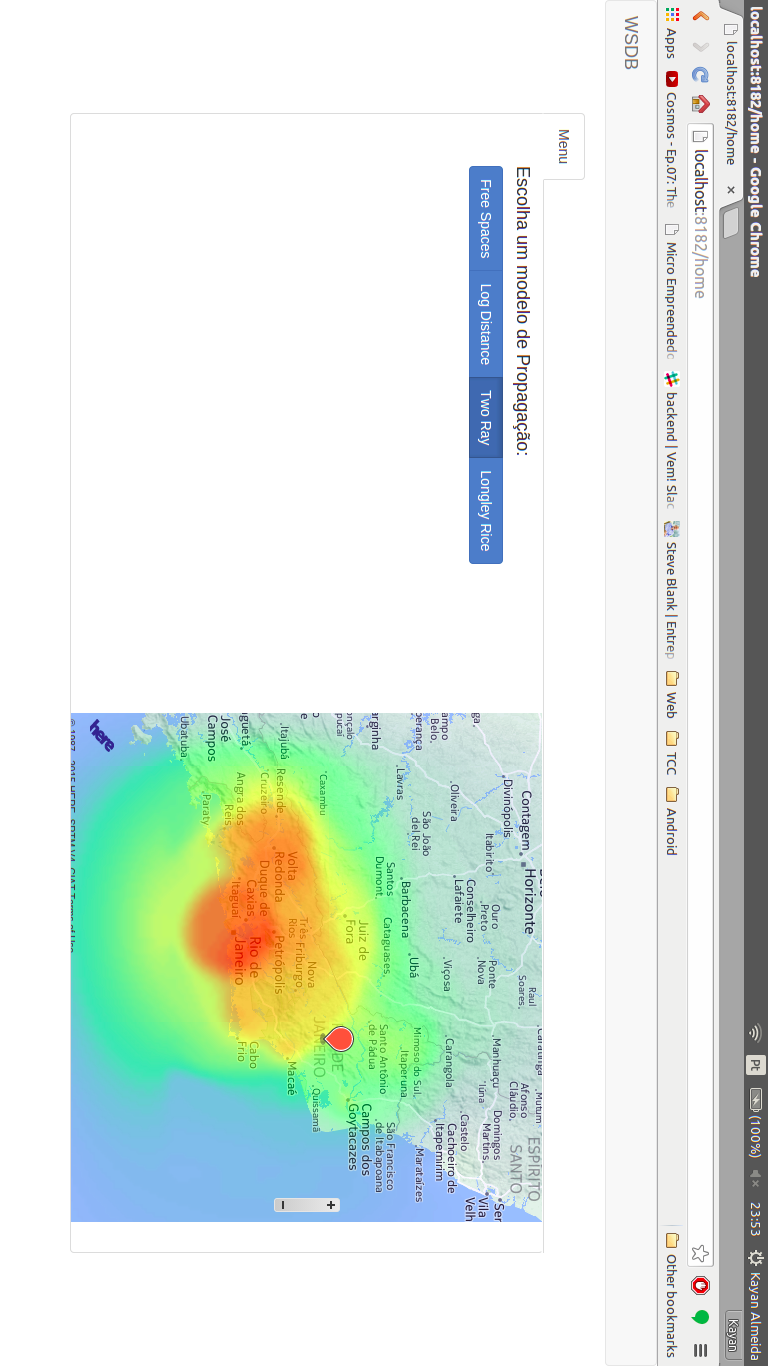
\includegraphics[width=1\textwidth]{figs/paginaweb}
\caption[\textit{Layout} da página Web.]
{\textit{Layout} da página Web.}
\label{fig:paginaweb}
\end{figure}

\FloatBarrier

\subsection{Modelo Free Spaces}

A figura~\ref{fig:freespacesout} representa o mapa de calor gerado, representando a disponibilidade de canais utilizando o modelo Free Space. A figura~\ref{fig:freespacesin} representa o mapa de calor aumentando o seu zoom.

\begin{figure}[htb]
\centering
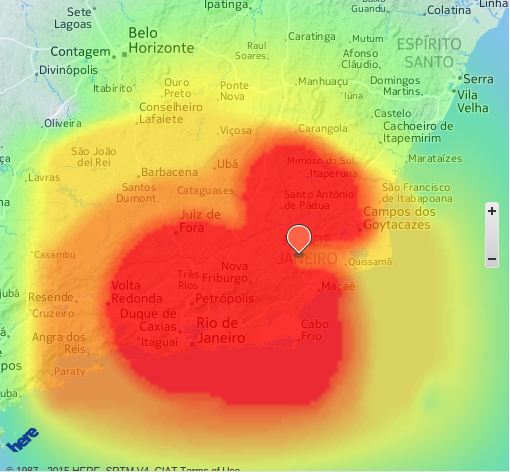
\includegraphics[width=1.0\textwidth]{figs/freespacesout}
\caption[Mapa de calor para o modelo Free Space]
{Mapa de calor para o modelo Free Space}
\label{fig:freespacesout}
\end{figure} 

\begin{figure}[htb]
\centering
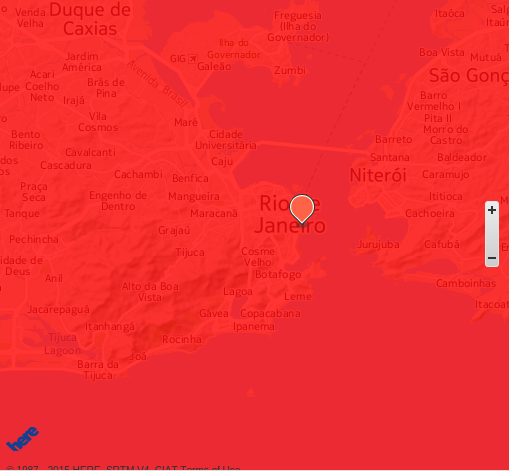
\includegraphics[width=1.0\textwidth]{figs/freespacesin}
\caption[Mapa de calor para o modelo Free Space com zoom]
{Mapa de calor para o modelo Free Space com zoom}
\label{fig:freespacesin}
\end{figure} 


\FloatBarrier

Como esperado, o espectro está bastante ocupado, pois o Free Spaces assume que não há obstáculos, portanto o raio de alcance da antena é muito grande. Com o máximo de 67 canais livres, mínimo de 8 e média de 9.08 canais.


\subsection{Modelo Log Distance}

A figura~\ref{fig:logdistanceout} representa o mapa de calor gerado, representando a disponibilidade de canais utilizando o modelo Log Distance constante de decaimento \begin{math}\alpha=3 \end{math}. A figura~\ref{fig:logdistancein} representa o mapa de calor aumentando o seu zoom.

\begin{figure}[htb]
\centering
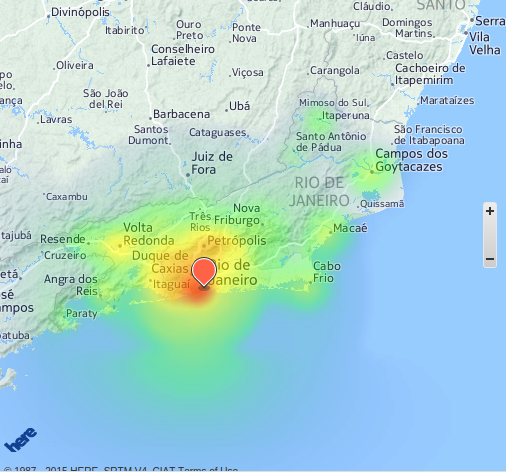
\includegraphics[width=1.0\textwidth]{figs/logdistanceout}
\caption[Mapa de calor para o modelo Log Distance]
{Mapa de calor para o modelo Log Distance}
\label{fig:logdistanceout}
\end{figure} 

\begin{figure}[htb]
\centering
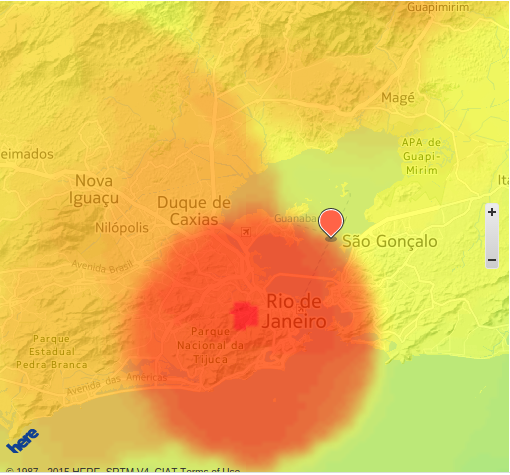
\includegraphics[width=1.0\textwidth]{figs/logdistancein}
\caption[Mapa de calor para o modelo Log Distance com zoom]
{Mapa de calor para o modelo Log Distance com zoom}
\label{fig:logdistancein}
\end{figure} 

\FloatBarrier

Como podemos observar, com o Log Distance o mapa fica mais compreensível. Nesse modelo, temos a média de 55.42 canais livres, com máximo de 67 e mínimo de 13 canais.

\subsection{Modelo Two Ray Ground}

A figura~\ref{fig:tworayout} representa o mapa de calor gerado, representando a disponibilidade de canais utilizando o modelo Free Space. A figura~\ref{fig:tworayin} representa o mapa de calor aumentando o seu zoom.

\begin{figure}[htb]
\centering
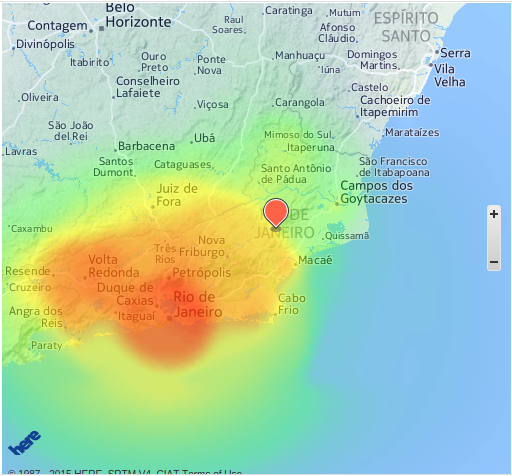
\includegraphics[width=1.0\textwidth]{figs/tworayout}
\caption[Mapa de calor para o modelo Two Ray Ground.]
{Mapa de calor para o modelo Two Ray Ground.}
\label{fig:tworayout}
\end{figure} 

\begin{figure}[htb]
\centering
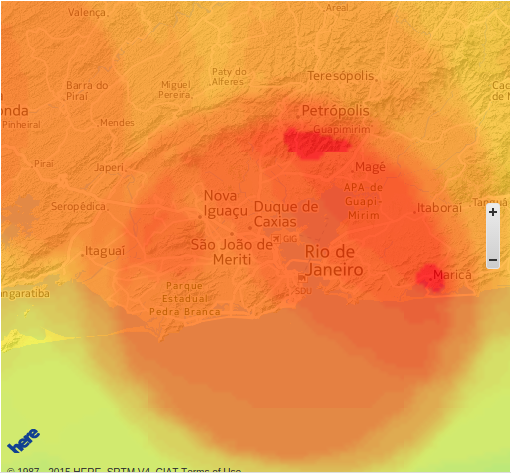
\includegraphics[width=1.0\textwidth]{figs/tworayin}
\caption[Mapa de calor para o modelo Two Ray Ground com zoom.]
{Mapa de calor para o modelo Two Ray Ground com zoom.}
\label{fig:tworayin}
\end{figure} 

\FloatBarrier

Esse modelo acusou uma média de 38.16 canais disponíveis por localização. Sendo 67 a quantidade máxima de canais disponíveis em uma localização e 10 a mínima.

\subsection{Modelo Longley-Rice}

A figura~\ref{fig:longleyriceout} representa o mapa de calor gerado, representando a disponibilidade de canais utilizando o modelo Free Space. A figura~\ref{fig:longleyricein} representa o mapa de calor aumentando o seu zoom.

\begin{figure}[htb]
\centering
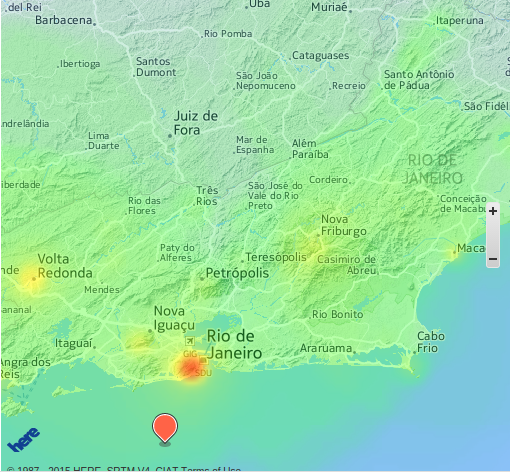
\includegraphics[width=1.0\textwidth]{figs/longleyriceout}
\caption[Mapa de calor para o modelo Two Ray Ground.]
{Mapa de calor para o modelo Two Ray Ground.}
\label{fig:longleyriceout}
\end{figure} 

\begin{figure}[htb]
\centering
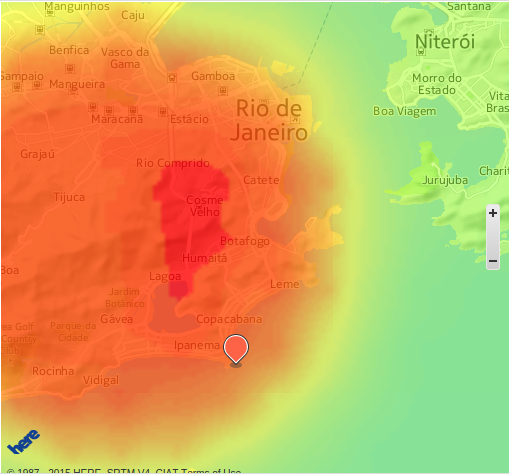
\includegraphics[width=1.0\textwidth]{figs/longleyricein}
\caption[Mapa de calor para o modelo Two Ray Ground com zoom.]
{Mapa de calor para o modelo Two Ray Ground com zoom.}
\label{fig:longleyricein}
\end{figure} 

\FloatBarrier

Esse modelo acusou uma média de 47.3 canais disponíveis por localização. Sendo 59 a quantidade máxima de canais disponíveis em uma localização e 16 a mínima.

\section{Resultado da análise}

\subsection{Diferença entre Modelos}

Como pode ser observado, de um modelo para o outro há diferenças significativas. O modelo a ser utilizado pela base deve ser o mais preciso possível.

Erros de precisão podem acarretar dois problemas: caso o modelo seja muito conservador, os alcances das antenas se tornam grandes demais, quando na realidade o canal pode ser usado por um rádio cognitivo. Isso gera uma subutilização do canal. O segundo problema pode ser para os modelos pouco sensíveis, fazendo com que o alcance da antena seja menor do que o real, gerando assim uma possível interferência caso um USs seja instalado na região.

Embora possa haver o desperdício, o ideal seria escolher um modelo um pouco conservador, para garantir que interferências não venham a ocorrer.

\subsubsection{Modelo Free Space}

O modelo Free Spaces foi o modelo em que os raios das antenas possuíam valores muito grandes. Com isso, é evidente que é o modelo mais sensível de todos os modelos apresentados, com a média pequena de canais livres.

\subsubsection{Log Distance}

O modelo Log Distance, com \begin{math}\alpha = 3 \end{math}, foi consideravelmente menos sensível que o modelo Free Spaces. Pode-se notar que os espaços urbanos possuem o espectro quase inteiramente ocupado, diferentemente das regiões menos povoadas.

\subsubsection{Two Ray}

O modelo Two Ray também é menos sensível que o Free Spaces, porém é mais conservador que o Log Distance. Ao levar em conta o sinal refletido na superfície, era esperado que fosse mais conservador. Porém, nota-se que o padrão é o mesmo que no modelo Log Distance, ou seja, as regiões urbanas possuem o espectro de frequência muito ocupado, em detrimento das regiões rurais.

\subsubsection{Longley-Rice}

O modelo Longley-Rice por sua vez, é o modelo menos conservador de todos. Por levar em conta as informações do terreno, a atenuação é consideravelmente maior. Nota-se o mesmo padrão dos modelos Two Ray e Log Distance para os espaços urbanos, porém o alcance das antenas é consideravelmente menor, por conta do relevo bastante acidentado do estado do Rio de Janeiro.

\subsection{Conclusão}

Dentre os modelos apresentados, o único que leva em conta o relevo é o Longley-Rice e o mesmo apresentou os melhores resultados. Como esperado, as regiões densamente povoadas, como centros urbanos, possuem um grau de disponibilidade muito baixo, ou seja, uma grande quantidade de usuários primários estão utilizando os canais. Porém, diferentemente dos outros modelos, o raio das antenas é menor, reduzindo assim o desperdício de canais livres. As áreas rurais por sua vez, possuem uma ampla quantidade de canais livres para uso.

Dos modelos estudados nesse trabalho, o modelo a ser utilizado por uma BDWS deve ser o Longley-Rice, modelo utilizado oficialmente pela FCC para cobertura de antenas de TV~\cite{fcclongleyrice}.

De maneira geral foi verificado que o Rio de Janeiro é uma área propícia para a implantação de rádios cognitivos. Embora as regiões metropolitanas já estejam densamente utilizadas, nota-se que a média de canais livres no estado é grande, de acordo com o Longley-Rice. Consequentemente, a utilização de dispositivos secundários visando descongestionar outros canais de transmissão, como o WiFi, pode ser realizada.
